%appendix.tex


    \section{Installing \LaTeXe}
    \label{Installing}

    \Lx{} formally consists of macros built on \TeX{}, a typesetting program created by Donald Knuth in the late 1970s. \Lx{} itself was create by Leslie Lamport in the early 1980s. Both \TeX{} and \Lx{} are open technologies, which means that anyone can implement them without restriction. Several implementations of \Lx{} are available, and opinions differ as to whichn one is ``best.'' I have tried several different implementations, and on Microsoft Windows, MiKTeX works best for me. You mileage may vary.
    
    This tutorial uses the MikTeX implementation of \Lx{}. MiKTeX's home (as of Auust, 2016) is \url{http://miktex.org/}. It can be downloaded by following the Download link (figure \ref{img:MiKTeX download}).  Typically, accepting the usual defaults will lead to a successful installation. In particular, the installation process will add the executable to your path, so youcan invoke kit without jumping through any hoops.

    If all goes well (and it should) you will see MiKTeX in your Windows start menu, as in figure \ref{img:MiKTeX winstart}. Note the program \texttt{TeXworks} --- you can use this as your \Lx{} development environment if you want, see appendix \ref{Development Environments}. You can also test your installation by executing the command \texttt{pdflatex --help} using your command line interface, see figure \ref{img:CLI test}.

    \begin{figure}[!hb]
        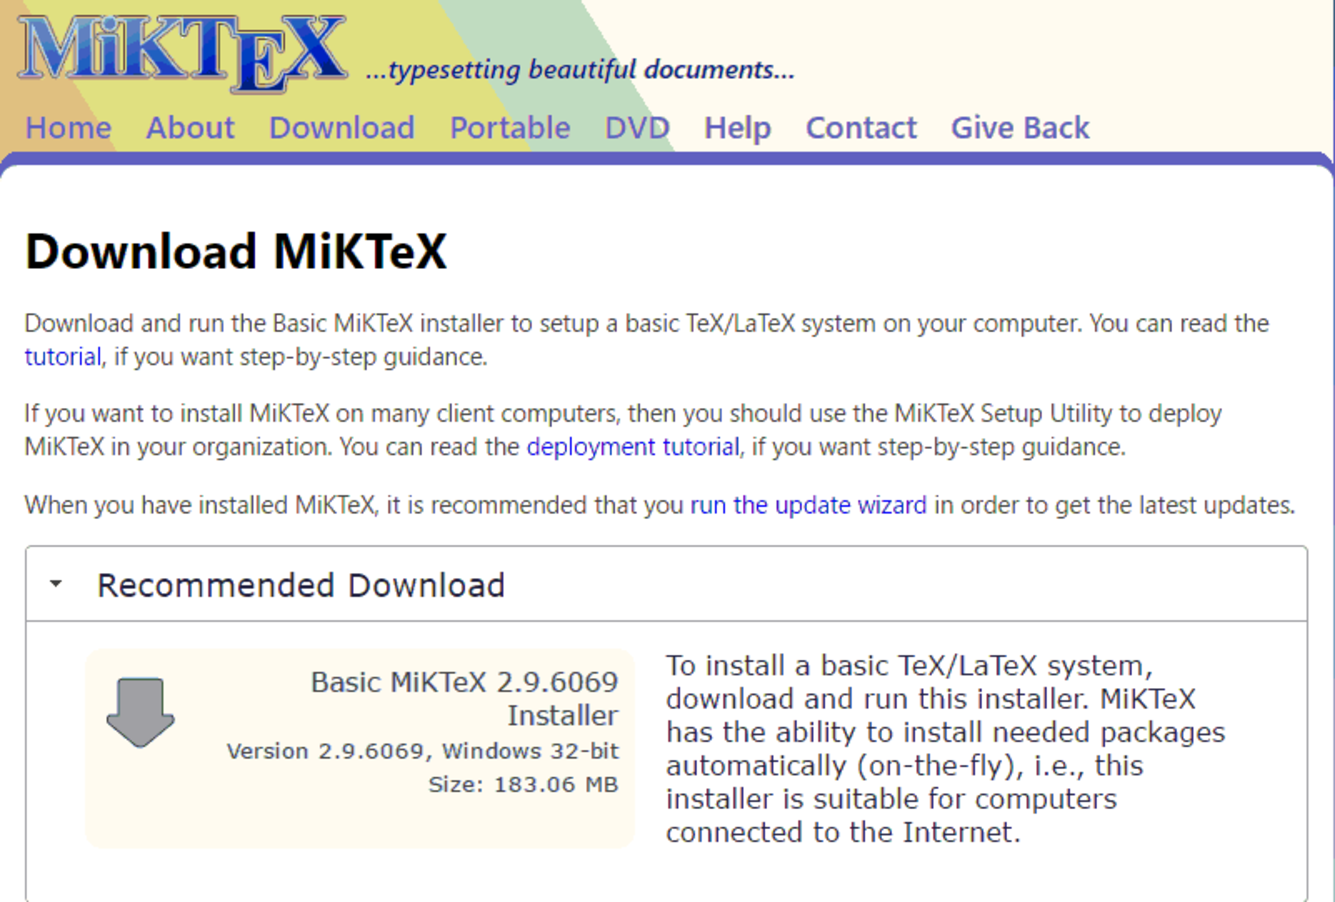
\includegraphics[width=3in]{images/miktex-download.pdf}
        \caption{MiKTeX download}
        \label{img:MiKTeX download}
    \end{figure}

    \begin{figure}[!hb]
        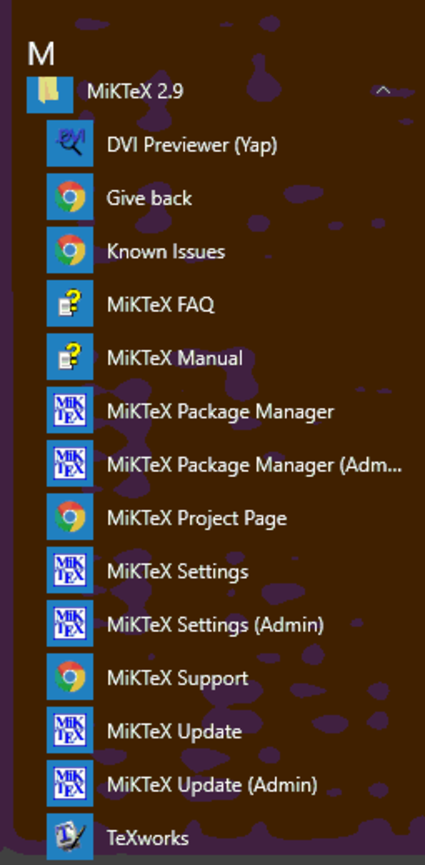
\includegraphics[width=1in]{images/miktex-winstart.pdf}
        \caption{MiKTeX on Windows start menu}
        \label{img:MiKTeX winstart}
    \end{figure}

    \begin{figure}[!hb]
        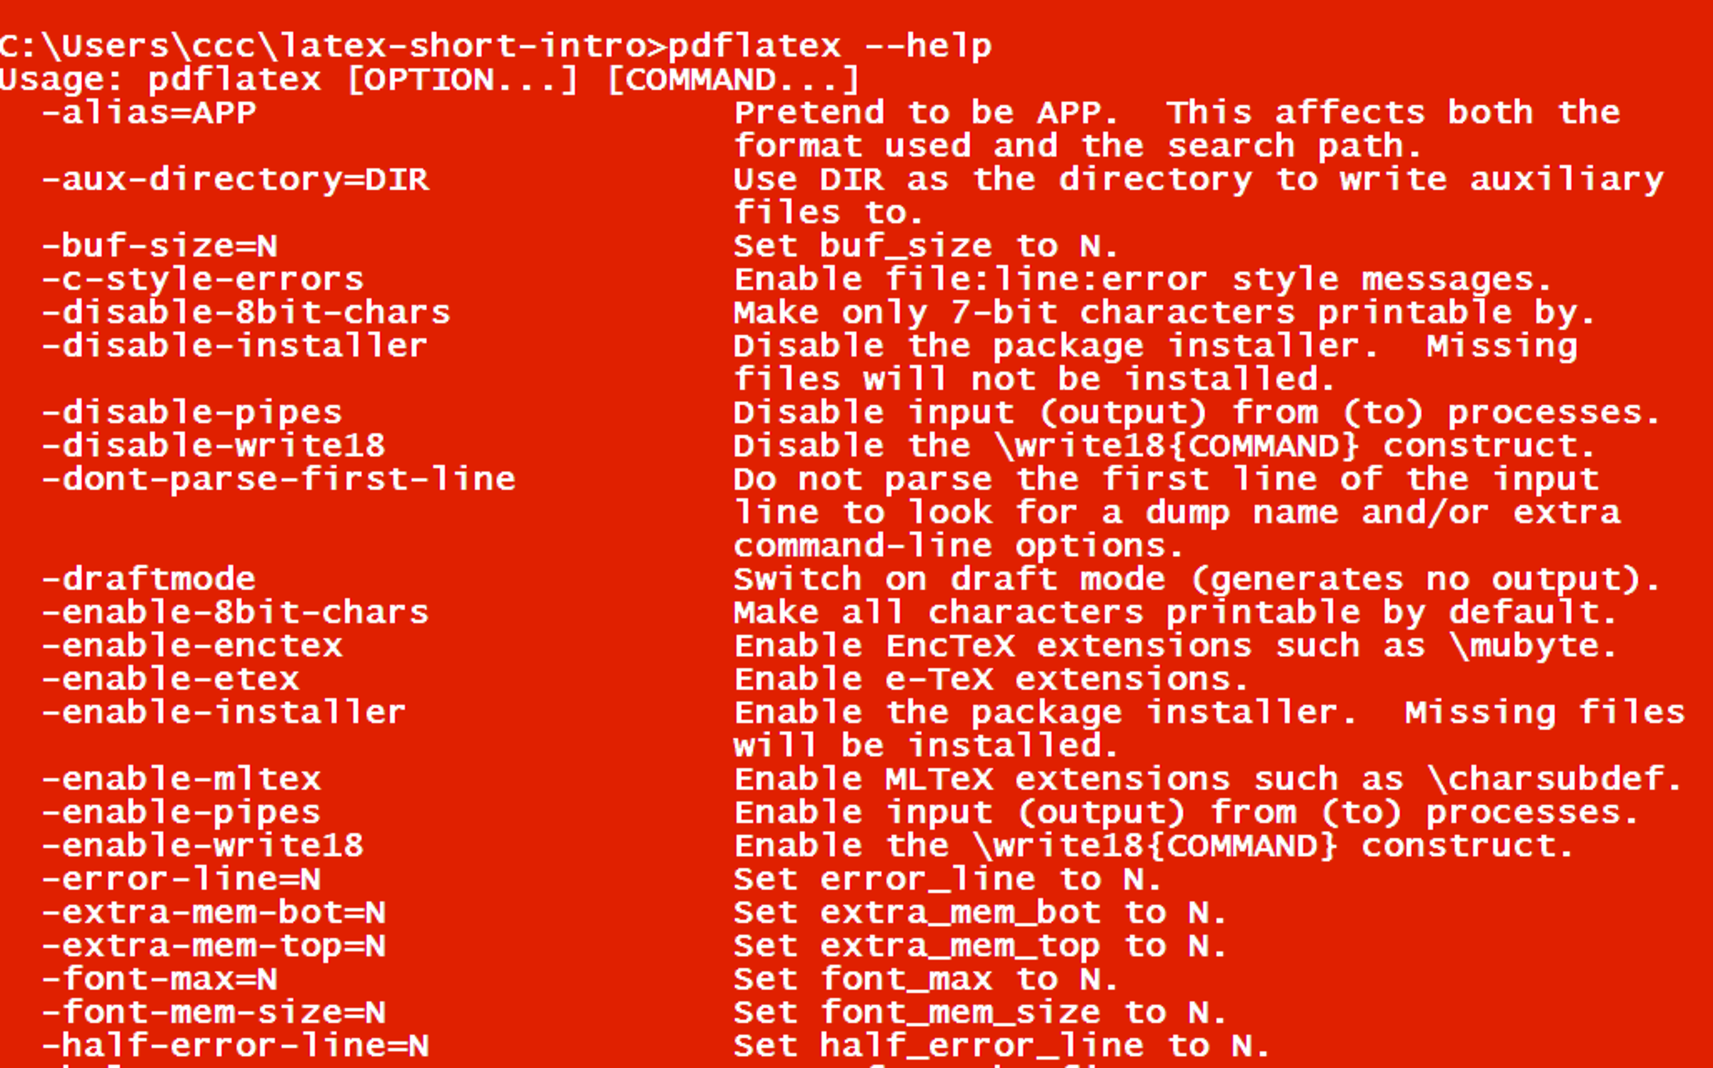
\includegraphics[width=3in]{images/install-test.pdf}
        \caption{CLI test}
        \label{img:CLI test}
    \end{figure}

    \section{\LaTeXe Editors}
    \label{Editors}

    A \texttt{tex} file is just ordinary plain text, without any special codes or binary commands. You write your \Lx{} document using an ordinary text editor. You can use your favorite text editor with no restrictions, from Windows Notepad (the most minimal text editor I know) on up.\footnote{But be careful of Notepad. Notepad by default saves documents with the \texttt{txt} extension, i.e., as a plain text file. You \textit{must} save your \Lx{} file with a \texttt{tex} extension. Be sure to select the All Files option in the Save As box, and explicitly add \texttt{.tex} to the name of your file}

    Notepad++ is a very popular, full featured, free text editor, and I recommend it for a large number of applications, including \Lx{}. You can find Notepad++ at \url{https://notepad-plus-plus.org/}. Notepad++ is just a text editor, so it doesn't come with any special bells and whistles.\footnote{If you really want to add a compilation feature to Notepad++, search the internet. It's not hard, but I don't cover it here.} Personally, I use \texttt{gvim} as my text editor, as it works for virtually everything, and works on Windows, Mac, Linux, and UNIX. However, \texttt{gvim} requires a substantial investment of time and effort to achieve proficiency, and I don't cover it here.

    Typically, a new user of \Lx{} will choose to use an integrated development which combines a text editor and compiler (see appendix \ref{Development Environments}) or an online resource (see appendix \ref{Online}). Use of a text editor requires separate editing and compilation cycles, which does offer some advantages, which is why some people choose to do it this way.

    \section{Development Environments}
    \label{Development Environments}

    MiKTeX comes with TeXwriter, which combines a text editor with a compiler. It's pretty minimal and crude, but that means that there's less to learn and less to break. Many other \Lx{} programs can be had, both free and commercial. Look at the Wikipedia entry on \Lx{} or \TeX{} editors. TeXmaker is also popular. The advantage to a development environment is that you can do your writing, editing, compilation, and publishing with one application. These also offer nice features, such as syntax coloring, autocomplete, and builtin help systems. The top end development environments also have point and click, drag and drop, features. This results in something close to a blend of a word processor (like Microsoft Word) and \Lx{}. Whether or not this is a good thing is a matter of opinion. You will find that people who use \Lx{} professionaly do not use these kinds of graphical interfaces --- there are very good reasons for this avoidance that you will come to see if you use \Lx{} frequently.

    \section{Online \LaTeXe}
    \label{Online}

    You can also use online \Lx{} editors. There are many equation editors that translate equations into \Lx{} source code. There are also full fledged online \Lx{} systems, which alalow collaboration between colleages. Many (virtually all) are commercial. I have never used any of these so I can't offer an opinion about them. If you do not have an adequate computer (such as a Chromebook, perhaps), online document writing is an option.

    \section{Command Line Execution}
    \label{Command Line}

    Both \TeX{} and \Lx{} consist of executable computer programs that can be invoked and executed on the command line. If you automate your processes (perhaps you have to create lengthy reports several times a day or a week) you will write programs that call these executables to produce your documents. The three commands you will use most often are \texttt{pdflatex}, \texttt{makeindex}, and \texttt{bibtex}. Power users commonly do their work on the command line, and again, there are good reasons for this.

    If the thought of the command line terrifies you, you never have to see it. However, it's always there lurking in the background. And sometimes, use of the command line is the only way to perform some tasks that your GUI program does not implement.

